%
% Copyright 2018 Joel Feldman, Andrew Rechnitzer and Elyse Yeager.
% This work is licensed under a Creative Commons Attribution-NonCommercial-ShareAlike 4.0 International License.
% https://creativecommons.org/licenses/by-nc-sa/4.0/
%
\graphicspath{{figures/roots/}}

\section{Roots of Polynomials}\label{ap:roots}
Being able to factor polynomials is a very important part of many of the computations in
this course. Related to this is the process of finding roots (or zeros) of polynomials.
That is, given a polynomial $P(x)$, find all numbers $r$ so that $P(r)=0$.

In the case of a quadratic $P(x)=ax^2+bx+c$, we can use the formula
\begin{align*}
  x &= \frac{-b \pm \sqrt{b^2-4ac}}{2a}
\end{align*}
The corresponding formulas for cubics and quartics\footnote{The method for cubics was
developed in the 15th century by del Ferro, Cardano and Ferrari (Cardano's
student). Ferrari then went on to discover a formula for the roots of a quartic. His
formula requires the solution of an associated cubic polynomial.}
are extremely cumbersome, and no such formula exists for polynomials of degree 5
and higher\footnote{This is the famous Abel-Ruffini theorem.}.

Despite this there are many tricks\footnote{There is actually a large body of
mathematics devoted to developing methods for factoring polynomials. Polynomial
factorisation is a fundamental problem for most computer algebra systems. The interested
reader should make use of their favourite search engine to find out more.} for finding
roots of polynomials that work well in some situations but not all. Here we describe
approaches that will help you find integer and rational roots of polynomials that will
work well on exams, quizzes and homework assignments.

Consider the quadratic equation $x^2 - 5x + 6=0$. We could\footnote{We probably
shouldn't do it this way for such a simple polynomial, but for pedagogical
purposes we do here.} solve this using the quadratic formula
\begin{align*}
  x &= \frac{5 \pm \sqrt{25-4\times1\times6}}{2} = \frac{5 \pm 1}{2} = 2,3.
\end{align*}
Hence  $x^2 - 5x + 6$ has roots $x = 2,3$ and so it factors as $(x - 3)(x -
2)$. Notice\footnote{Many of you may have been taught this approach in
highschool.} that the numbers $2$ and $3$ divide the constant term of the
polynomial, $6$. This happens in general and forms the basis of our first trick.

\begin{trick}[A very useful trick]
If $r$ or $-r$ is an integer root of a polynomial
$P(x)=a_nx^n+\ \cdots\ +a_1x+a_0$ with integer coefficients, then $r$ is a factor
of the constant term $a_0$.
\end{trick}

\begin{proof}
If $r$ is a root of the polynomial we know that $P(r)=0$. Hence
\begin{align*}
  a_n \cdot r^n+\ \cdots\ +a_1\cdot r+a_0&=0
\end{align*}
If we isolate $a_0$ in this expression we get
\begin{align*}
  a_0 &=-\big[a_n r^n+\ \cdots\ +a_1r\big]
\end{align*}
We can see that $r$ divides every term on the right-hand side. This means that the
right-hand side is an integer times $r$. Thus the left-hand side, being $a_0$, is an
integer times $r$, as required. The argument for when $-r$ is a root is almost identical.
\end{proof}

Let us put this observation to work.
\begin{eg}
Find the integer roots of $P(x)=x^3-x^2+2$.

\soln
\begin{itemize}
 \item The constant term in this polynomial is $2$.
 \item The only divisors of $2$ are $1,2$. So the only candidates
for integer roots are $\pm 1, \pm 2$.
\item Trying each in turn
\begin{align*}
P(1)&=2 & P(-1)&=0 \\
P(2)&=6 & P(-2) &=-10
\end{align*}
\item Thus the only integer root is $-1$.
\end{itemize}
\end{eg}

\begin{eg}
 Find the integer roots of $P(x)= 3x^3+8x^2-5x-6$.

\soln
\begin{itemize}
 \item The constant term is $-6$.
\item The divisors of $6$ are $1,2,3,6$. So the only candidates for integer roots are
$\pm1, \pm 2, \pm 3, \pm 6$.
\item We try each in turn (it is tedious but not difficult):
\begin{align*}
  P(1) &= 0 & P(-1) &= 4 \\
  P(2) &= 40 & P(-2) &= 12\\
  P(3) &= 132 & P(-3) &= 0\\
  P(6) &= 900 & P(-6) &= -336
\end{align*}
\item Thus the only integer roots are $1$ and $-3$.
\end{itemize}
\end{eg}

We can generalise this approach in order to find rational roots. Consider the polynomial
$6x^2-x-2$. We can find its zeros using the quadratic formula:
\begin{align*}
 x &= \frac{1 \pm \sqrt{1 + 48}}{12} = \frac{1\pm 7}{12} = -\frac{1}{2}, \frac{2}{3}.
\end{align*}
Notice now that the numerators, 1 and 2, both divide the constant term of the polynomial
(being 2). Similarly, the denominators, 2 and 3, both divide the coefficient of the
highest power of $x$ (being 6). This is quite general.

\begin{trick}[Another nice trick]
If $b/d$ or $-b/d$ is a rational root in lowest terms (i.e. $b$ and $d$
are integers with no common factors) of a polynomial
$Q(x) = a_nx^n+\ \cdots\ +a_1x+a_0$ with integer coefficients, then the numerator
$b$ is a factor of the constant term $a_0$ and the denominator $d$ is a
factor of $a_n$.
\end{trick}

\begin{proof}
Since $\nicefrac{b}{d}$ is a root of $P(x)$ we know that
\begin{align*}
a_n(b/d)^n+\ \cdots\ +a_1(b/d)+a_0 &=0
\end{align*}
Multiply this equation through by $d^n$ to get
\begin{align*}
a_n b^n+\ \cdots\ +a_1 b d^{n-1}+a_0d^n &=0
\end{align*}
Move terms around to isolate $a_0 d^n$:
\begin{align*}
  a_0d^n &= - \big[ a_n b^n+\ \cdots\ +a_1 b d^{n-1} \big]
\end{align*}
Now every term on the right-hand side is some integer times $b$. Thus the left-hand side
must also be an integer times $b$. We know that $d$ does not contain any factors of $b$,
hence $a_0$ must be some integer times $b$ (as required).

Similarly we can isolate the term $a_n b^n$:
\begin{align*}
  a_n b^n &= - \big[ a_{n-1} b^{n-1}d+\ \cdots\ +a_1 b d^{n-1} + a_0 d^n \big]
\end{align*}
Now every term on the right-hand side is some integer times $d$. Thus the left-hand side
must also be an integer times $d$. We know that $b$ does not contain any factors of $d$,
hence $a_n$ must be some integer times $d$ (as required).

The argument when $-\nicefrac{b}{d}$ is a root is nearly identical.
\end{proof}


We should put this to work:
\begin{eg}
$P(x)=2x^2-x-3$.

\soln
\begin{itemize}
 \item The constant term in this polynomial is $3=1\times 3$ and the coefficient
of the highest power of $x$ is $2=1\times 2$.
\item Thus the only candidates for integer roots are $\pm 1,\ \pm 3$.
\item By our newest trick, the only candidates for fractional
roots are $\pm \frac{1}{2},\ \pm\frac{3}{2}$.
\item We try each in turn\footnote{Again, this is a little tedious, but not
difficult. Its actually pretty easy to code up for a computer to do. Modern
polynomial factoring algorithms do more sophisticated things, but these are a
pretty good way to start.}
\begin{align*}
P(1)&=-2 & P(-1)&=0 \\
P(3)&=12 & P(-3)&=18\\
P\left(\tfrac{1}{2}\right) &= -3 &
P\left(-\tfrac{1}{2}\right) &= -2 \\
P\left(\tfrac{3}{2}\right) &= 0 &
P\left(-\tfrac{3}{2}\right) &= 3
% P\big(\pm\tfrac{1}{2})=2\tfrac{1}{4}\mp\half-3\ne 0  &
% &P\big(\tfrac{3}{2})=2\tfrac{9}{4}-\tfrac{3}{2}-3=0  &
% &P\big(-\tfrac{3}{2})=2\tfrac{9}{4}+\tfrac{3}{2}-3\ne 0
\end{align*}
so the roots are $-1$ and $\frac{3}{2}$.
\end{itemize}
\end{eg}

The tricks above help us to find integer and rational roots of polynomials. With a little
extra work we can extend those methods to help us factor polynomials. Say we have a
polynomial $P(x)$ of degree $p$ and have established that $r$ is one of its
roots. That is, we know $P(r)=0$. Then we can factor $(x-r)$ out from
$P(x)$ --- it is always possible to find a polynomial $Q(x)$ of degree $p-1$ so
that
\begin{align*}
  P(x) = (x-r)Q(x)
\end{align*}

In sufficiently simple cases, you can probably do this factoring by
inspection. For example, $P(x)=x^2-4$ has $r=2$ as a root because
$P(2)=2^2-4=0$.  In this case, $P(x)=(x-2)(x+2)$ so that
$Q(x)=(x+2)$. As another example, $P(x)=x^2-2x-3$ has $r=-1$ as a root
because $P(-1)=(-1)^2-2(-1)-3=1+2-3=0$. In this case,
$P(x)=(x+1)(x-3)$ so that $Q(x)=(x-3)$.

% We can also make the above more explicit.
% \begin{eg}
% Say we have $P(x)=x^3+3x^2+4x+2$ and we know
% that $r=-1$ is a root. Then we know that $P(x)=(x+1)Q(x)$ where $Q(x)$ must have degree
% 2. Write $Q(x)$ explicitly as $ax^2+bx+c$. Then
% \begin{align*}
%   P(x) &= x^3+3x^2+4x+2 \\
%   &= (x+1)(ax^2+bx+c) & \text{expand it out}\\
%   &= ax^3 + x^2(a+b) + x(b+c) +c
% \end{align*}
% Then by comparing coefficients of $x$ we know that $a=1,a+b=3,b+c=4,c=2$. Hence $b=2$ and
% \begin{align*}
%   x^3+3x^2-2x-3 &= (x+1)(x^2+2x+2).
% \end{align*}
% \end{eg}

For higher degree polynomials we need to use something more systematic --- long
divison.
\begin{trick}[Long Division]
Once you have found a root $r$ of a polynomial, even if you cannot factor
$(x-r)$ out of the polynomial by inspection, you can find $Q(x)$
by dividing $P(x)$ by $x-r$, using the long division algorithm you learned\footnote{This
is a standard part of most highschool mathematics curricula, but perhaps not all. You
should revise this carefully.} in school, but with $10$ replaced by $x$.
\end{trick}

\begin{eg}
Factor $P(x)=x^3-x^2+2$.

\soln
\begin{itemize}
 \item We can go hunting for integer roots of the polynomial by looking at the divisors
of the constant term. This tells us to try $x=\pm1, \pm2$.
\item A quick computation shows that $P(-1)=0$ while $P(1),P(-2),P(2) \neq 0$. Hence
$x=-1$ is a root of the polynomial and so $x+1$ must be a factor.
\item  So we divide  $\frac{x^3-x^2+2}{x+1}$. The first term, $x^2$, in the quotient
is chosen so that when you multiply it by the  denominator,
$x^2(x+1)=x^3+x^2$, the leading term, $x^3$,  matches the leading term
in the numerator, $x^3-x^2+2$, exactly.
\begin{center}
  
\includegraphics{longdiv2}
\end{center}
\item When you subtract $x^2(x+1)=x^3+x^2$ from the numerator $x^3-x^2+2$ you
get the remainder $-2x^2+2$. Just like in public school, the $2$ is
not normally ``brought down'' until it is actually needed.
\begin{center}
  
\includegraphics{longdiv3}
\end{center}
\item The next term, $-2x$, in the quotient is chosen so that when you multiply
it by the  denominator, $-2x(x+1)=-2x^2-2x$, the leading term
$-2x^2$  matches the leading term in the remainder exactly.
\begin{center}
  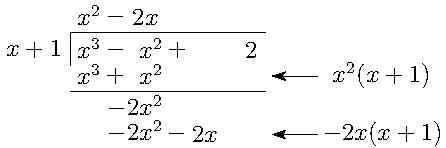
\includegraphics{longdiv4}
\end{center}
And so on.
\begin{center}
  
\includegraphics{longdiv5}
\end{center}
\item  Note that we finally end up with a remainder $0$. A nonzero remainder
would have signalled a computational error, since we know that the
denominator $x-(-1)$ must divide the numerator $x^3-x^2+2$ exactly.
\item We conclude that
\begin{align*}
(x+1)(x^2-2x+2)=x^3-x^2+2
\end{align*}
To check this, just multiply out the left hand side explicitly.

% \item We can then reapply our tricks to $x^2-2x+2$ and examine $x=\pm1, \pm2$.
% None of these are roots, and so we can conclude that the polynomial does not
% factor further\footnote{To be more precise, it does not factor further over the
% rational numbers.}.

\item Applying the high school quadratic root formula
$\frac{-b\pm\sqrt{b^2-4ac}}{2a}$ to $x^2-2x+2$ tells us that it has no real
roots and that we cannot factor it further\footnote{Because we are not permitted
to use complex numbers.}.
\end{itemize}
\end{eg}

We finish by describing an alternative to long division. The approach is roughly
equivalent, but is perhaps more straightforward at the expense of requiring
more algebra.
\begin{eg}
Factor $P(x)=x^3-x^2+2$, again.

\soln Let us do this again but avoid long division.
\begin{itemize}
 \item From the previous example, we know that  $\frac{x^3-x^2+2}{x+1}$ must
be a polynomial (since $-1$ is a root of the numerator) of degree 2. So write
\begin{align*}
\frac{x^3-x^2+2}{x+1}=ax^2+bx+c
\end{align*}
for some, as yet unknown, coefficients $a,\ b$ and $c$.
\item Cross multiplying and simplifying gives us
\begin{align*}
x^3-x^2+2&=(ax^2+bx+c)(x+1)\\
&=ax^3+(a+b)x^2+(b+c)x+c
\end{align*}
\item Now matching coefficients of the various powers of $x$ on the left and right
hand sides
\begin{alignat*}{3}
&\text{coefficient of $x^3$:}\qquad&a&=1\\
&\text{coefficient of $x^2$:}&a+b&=-1\\
&\text{coefficient of $x^1$:}& b+c&=0\\
&\text{coefficient of $x^0$:}& c&=2
\end{alignat*}
\item This gives us a system of equations that we can solve quite directly. Indeed it
tells us immediately that that $a=1$ and $c=2$. Subbing $a=1$ into $a+b=-1$ tells us
that $1+b=-1$ and hence $b=-2$.
\item Thus
\begin{align*}
x^3-x^2+2 &= (x+1)(x^2-2x+2).
\end{align*}
\end{itemize}
\end{eg}
